% defer/rcuintro.tex
% mainfile: ../perfbook.tex
% SPDX-License-Identifier: CC-BY-SA-3.0

\subsection{Introduction to RCU}
\label{sec:defer:Introduction to RCU}

The approaches discussed in the preceding sections have provided
good scalability but decidedly non-ideal performance for the
Pre-BSD routing table.
Therefore, in the spirit of ``only those who have gone too far
know how far you can go'',\footnote{
	With apologies to T.~S.~Eliot.}
we will go all the way, looking into algorithms in which concurrent
readers execute the same sequence of assembly language instructions as
would a single-threaded lookup, despite the presence of concurrent
updates.
Of course, this laudable goal might raise serious implementability
questions, but we cannot possibly succeed if we don't even try!

\subsubsection{Minimal Insertion and Deletion}
\label{sec:defer:Minimal Insertion and Deletion}

\begin{figure}
\centering
\resizebox{3in}{!}{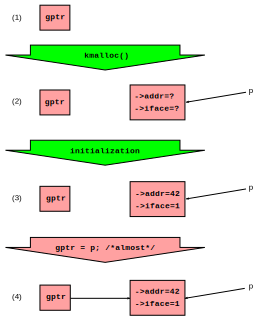
\includegraphics{defer/RCUListInsertClassic}}
\caption{Insertion With Concurrent Readers}
\label{fig:defer:Insertion With Concurrent Readers}
\end{figure}

To minimize implementability concerns, we focus on a minimal
data structure, which consists of a single global pointer that is either
\co{NULL} or references a single structure.
Minimal though it might be, this data structure is heavily used in
production~\cite{GeoffRomer2018C++DeferredReclamationP0561R4}.
A classic approach for insertion is shown in
\cref{fig:defer:Insertion With Concurrent Readers},
which shows four states with time advancing from top to bottom.
The first row shows the initial state, with \co{gptr} equal to \co{NULL}.
In the second row, we have allocated a structure which is uninitialized,
as indicated by the question marks.
In the third row, we have initialized the structure.
Finally, in the fourth and final row, we have updated \co{gptr} to
reference the newly allocated and initialized element.

We might hope that this assignment to \co{gptr} could use a simple
C-language assignment statement.
Unfortunately,
\cref{sec:toolsoftrade:Shared-Variable Shenanigans}
dashes these hopes.
Therefore, the updater cannot use a simple C-language assignment, but
must instead use \co{smp_store_release()} as shown in the figure,
or, as will be seen, \co{rcu_assign_pointer()}.

Similarly, one might hope that readers could use a single C-language
assignment to fetch the value of \co{gptr}, and be guaranteed to either
get the old value of \co{NULL} or to get the newly installed pointer,
but either way see a valid result.
Unfortunately, \cref{sec:toolsoftrade:Shared-Variable Shenanigans}
dashes these hopes as well.
To obtain this guarantee, readers must instead use \co{READ_ONCE()},
or, as will be seen, \co{rcu_dereference()}.
However, on most modern computer systems, each of these read-side primitives
can be implemented with a single load instruction, exactly the instruction
that would normally be used in single-threaded code.

Reviewing \cref{fig:defer:Insertion With Concurrent Readers}
from the viewpoint of readers, in the first three states all readers
see \co{gptr} having the value \co{NULL}.
Upon entering the fourth state, some readers might see \co{gptr} still
having the value \co{NULL} while others might see it referencing the
newly inserted element, but after some time, all readers will see this
new element.
At all times, all readers will see \co{gptr} as containing a valid pointer.
Therefore, it really is possible to add new data to linked data structures
while allowing concurrent readers to execute the same sequence of machine
instructions that is normally used in single-threaded code.
This no-cost approach to concurrent reading provides excellent performance
and scalability, and also is eminently suitable for real-time use.

\begin{figure}
\centering
\resizebox{3in}{!}{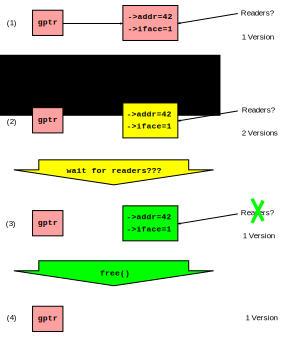
\includegraphics{defer/RCUListDeleteClassic}}
\caption{Deletion With Concurrent Readers}
\label{fig:defer:Deletion With Concurrent Readers}
\end{figure}

Insertion is of course quite useful, but sooner or later, it will also
be necessary to delete data.
As can be seen in
\cref{fig:defer:Deletion With Concurrent Readers},
the first step is easy.
Again taking the lessons from
\cref{sec:toolsoftrade:Shared-Variable Shenanigans}
to heart, \co{smp_store_release()} is used to \co{NULL} the pointer,
thus moving from the first row to the second in the figure.
At this point, pre-existing readers see the old structure with
\co{->addr} of 42 and \co{->iface} of 1, but new readers will see
a \co{NULL} pointer, that is, concurrent readers can disagree on
the state, as indicated by the ``2 Versions'' in the figure.

\QuickQuizSeries{%
\QuickQuizB{
	Why does
	\cref{fig:defer:Deletion With Concurrent Readers}
	use \co{smp_store_release()} given that it is storing
	a \co{NULL} pointer?
	Wouldn't \co{WRITE_ONCE()} work just as well in this case,
	given that there is no structure initialization to order
	against the store of the \co{NULL} pointer?
}\QuickQuizAnswerB{
	Yes, it would.

	Because a \co{NULL} pointer is being assigned, there is nothing
	to order against, so there is no need for \co{smp_store_release()}.
	In contrast, when assigning a non-\co{NULL} pointer, it is
	necessary to use \co{smp_store_release()} in order to ensure
	that initialization of the pointed-to structure is carried
	out before assignment of the pointer.

	In short, \co{WRITE_ONCE()} would work, and would
	save a little bit of CPU time on some architectures.
	However, as we will see, software-engineering concerns
	will motivate use of a special \co{rcu_assign_pointer()}
	that is quite similar to \co{smp_store_release()}.
}\QuickQuizEndB
%
\QuickQuizE{
	Readers running concurrently each other and with the procedure
	outlined in
	\cref{fig:defer:Deletion With Concurrent Readers}
	can disagree on the value of \co{gptr}.
	Isn't that just a wee bit problematic???
}\QuickQuizAnswerE{
	Not necessarily.

	As hinted at in
	\cref{sec:cpu:Hardware Optimizations,sec:cpu:Hardware Free Lunch?},
	speed-of-light delays mean that a computer's data is always
	stale compared to whatever external reality that data is intended
	to model.

	Real-world algorithms therefore absolutely must tolerate
	inconsistancies between external reality and the in-computer
	data reflecting that reality.
	Many of those algorithms are also able to tolerate some degree
	of inconsistency within the in-computer data.
	\Cref{sec:datastruct:RCU-Protected Hash Table Discussion}
	discusses this point in more detail.

	Please note that this need to tolerate inconsistent and stale
	data is not limited to RCU\@.
	It also applies to reference counting, hazard pointers, sequence
	locks, and even to some locking use cases.
	For example, if you compute some quantity while holding a lock,
	but use that quantity after releasing that lock,
	you might well be using stale data.
	After all, the data that quantity is based on might change
	arbitrarily as soon as the lock is released.

	So yes, RCU readers can see stale and inconsistent data, but no,
	this is not necessarily problematic.
	And, when needed, there are RCU usage patterns that avoid both
	staleness and inconsistency~\cite{Arcangeli03}.
}\QuickQuizEndE
}

We get back to a single version simply by waiting for all the
pre-existing readers to complete, as shown in row~3.
At that point, all the pre-existing readers are done, and no later
reader has a path to the old data item, so there can no longer be
any readers referencing it.
It may therefore be safely freed, as shown on row~4.

Thus, given a way to wait for pre-existing readers to complete,
it is possible to both add data to and remove data from a linked
data structure, despite the readers executing the same sequence
of machine instructions that would be appropriate for single-threaded
execution.
So perhaps going all the way was not too far after all!

But how can we tell when all of the pre-existing readers have in
fact completed?
This question is the topic of the \cref{sec:defer:Waiting for Readers}.
But first, the next section defines RCU's core API.

\subsubsection{Core RCU API}
\label{sec:defer:Core RCU API}

The full Linux-kernel API is quite extensive, with more than one
hundred API members.
However, this section will confine itself to six core RCU API members,
which suffices for the upcoming sections introducing RCU and covering
its fundamentals.
The full API is covered in \cref{sec:defer:RCU Linux-Kernel API}.

Three members of the core APIs are used by readers.
The \apik{rcu_read_lock()} and \apik{rcu_read_unlock()} functions delimit
RCU read-side critical sections.
These may be nested, so that one \co{rcu_read_lock()}-\co{rcu_read_unlock()}
pair can be enclosed within another.
In this case, the nested set of RCU read-side critical section act as
one large critical section covering the full extent of the nested set.
The third read-side API member, \apik{rcu_dereference()}, fetches an
RCU-protected pointer.
Conceptually, \co{rcu_dereference()} simply loads from memory, but we
will see in
\cref{sec:defer:Publish-Subscribe Mechanism}
that \co{rcu_dereference()} must prevent the compiler and (in
one case) the CPU from reordering its load with later memory operations
that dereference this pointer.

The other three members of the core APIs are used by updaters.
The \apik{synchronize_rcu()} function implements the ``wait for readers''
operation from \cref{fig:defer:Deletion With Concurrent Readers}.
The \apik{call_rcu()} function is the asynchronous counterpart of
\co{synchronize_rcu()} by invoking the specified function after
all pre-existing RCU readers have completed.
Finally, the \apik{rcu_assign_pointer()} macro is used to update an
RCU-protected pointer.
Conceptually, this is simply an assignment statement, but we will
see in
\cref{sec:defer:Publish-Subscribe Mechanism}
that \co{rcu_assign_pointer()} must prevent the compiler and the CPU
from reordering this assignment to precede any prior assignments used
to initialize the pointed-to structure.

\QuickQuiz{
	What does \co{synchronize_rcu()} do if it starts at about
	the same time as an \co{rcu_read_lock()}?
}\QuickQuizAnswer{
	If a \co{synchronize_rcu()} cannot prove that it started
	before a given \co{rcu_read_lock()}, then it must wait
	for the corresponding \co{rcu_read_unlock()}.
}\QuickQuizEnd

\begin{table*}
\renewcommand*{\arraystretch}{1.25}
\rowcolors{2}{}{lightgray}
\small
\centering
\ebresizewidth{
\begin{tabular}{llp{2.4in}}
\toprule
&
	Primitive &
		Purpose \\
\midrule
\cellcolor{white}\emph{Readers} &
	\tco{rcu_read_lock()} &
		Start an RCU read-side critical section. \\
&
	\tco{rcu_read_unlock()} &
		End an RCU read-side critical section. \\
\cellcolor{white}&
	\tco{rcu_dereference()} &
		Safely load an RCU-protected pointer. \\
\midrule
\emph{Updaters} &
	\tco{synchronize_rcu()} &
		Wait for all pre-existing RCU read-side critical sections to
		complete. \\
\cellcolor{white}&
	\tco{call_rcu()} &
		Invoke the specified function after all pre-existing RCU read-side
		critical sections complete. \\
&
	\tco{rcu_assign_pointer()} &
		Safely update an RCU-protected pointer. \\
\bottomrule
\end{tabular}
}
\caption{RCU Core API}
\label{tab:defer:RCU Core API}
\end{table*}

The core RCU API is summarized in \cref{tab:defer:RCU Core API} for
easy reference.
With that, we are ready to continue this introduction to RCU with
the key RCU operation, waiting for readers.

\subsubsection{Waiting for Readers}
\label{sec:defer:Waiting for Readers}

It is tempting to base the reader-waiting functionality of
\co{synchronize_rcu()} and \co{call_rcu()} on a reference counter
updated by \co{rcu_read_lock()} and \co{rcu_read_unlock()}, but
\cref{fig:count:Atomic Increment Scalability on x86}
in
\cref{chp:Counting}
shows that concurrent reference counting results in extreme overhead.
This extreme overhead was confirmed in the specific case of
reference counters in
\cref{fig:defer:Pre-BSD Routing Table Protected by Reference Counting}
on
\cpageref{fig:defer:Pre-BSD Routing Table Protected by Reference Counting}.
Hazard pointers profoundly reduce this overhead, but, as we saw in
\cref{fig:defer:Pre-BSD Routing Table Protected by Hazard Pointers}
on
\cpageref{fig:defer:Pre-BSD Routing Table Protected by Hazard Pointers},
not to zero.
Nevertheless, many RCU implementations make very careful cache-local
use of counters.

A second approach observes that memory synchronization is expensive,
and therefore uses registers instead, namely each CPU's or thread's
program counter (PC), thus imposing no overhead on readers, at least
in the absence of concurrent updates.
The updater polls each relevant PC, and if that PC is not within read-side
code, then the corresponding CPU or thread is within a quiescent state,
in turn signaling the completion of any reader that might have access
to the newly removed data element.
Once all CPU's or thread's PCs have been observed to be outside of any
reader, the \IX{grace period} has completed.
Please note that this approach poses some serious challenges, including
memory ordering, functions that are \emph{sometimes} invoked from readers,
and ever-exciting code-motion optimizations.
Nevertheless, this approach is said to be used in
production~\cite{MikeAsh2015Apple}.

A third approach is to simply wait for a fixed period of time that is
long enough to comfortably exceed the lifetime of any reasonable
reader~\cite{Jacobson93,AjuJohn95}.
This can work quite well in hard real-time systems~\cite{YuxinRen2018RTRCU},
but in less exotic
settings, Murphy says that it is critically important to be prepared
even for unreasonably long-lived readers.
To see this, consider the consequences of failing do so:
A data item will be freed while the unreasonable reader is still
referencing it, and that item might well be immediately reallocated,
possibly even as a data item of some other type.
The unreasonable reader and the unwitting reallocator would then
be attempting to use the same memory for two very different purposes.
The ensuing mess will at best be exceedingly difficult to debug.

A fourth approach is to wait forever, secure in the knowledge that
doing so will accommodate even the most unreasonable reader.
This approach is also called ``leaking memory'', and has a bad reputation
due to the fact that memory leaks often require untimely and
inconvenient reboots.
Nevertheless, this is a viable strategy when the update rate and the
uptime are both sharply bounded.
For example, this approach could work well in a high-availability
cluster where systems were periodically crashed in order to ensure
that cluster really remained highly available.\footnote{
	The program that forces the periodic crashing is sometimes
	known as a ``chaos monkey'':
	\url{https://netflix.github.io/chaosmonkey/}.
	However, it might also be a mistake to neglect chaos caused
	by systems running for too long.}
Leaking the memory is also a viable strategy in environments having
garbage collectors, in which case the garbage collector can be thought
of as plugging the leak~\cite{Kung80}.
However, if your environment lacks a garbage collector, read on!

A fifth approach avoids the period crashes in favor of periodically
``stopping the world'', as exemplified by the traditional stop-the-world
garbage collector.
This approach was also heavily used during the decades before
ubiquitous connectivity, when it was common practice to power systems
off at the end of each working day.
However, in today's always-connected always-on world, stopping the world
can gravely degrade response times, which has been one motivation for the
development of concurrent garbage collectors~\cite{DavidFBacon2003RTGC}.
Furthermore, although we need all pre-existing readers to complete, we do
not need them all to complete at the same time.

This observation leads to the sixth approach, which is stopping
one CPU or thread at a time.
This approach has the advantage of not degrading reader response times
at all, let alone gravely.
Furthermore, numerous applications already have states (termed
\emph{\IXpl{quiescent state}}) that can be
reached only after all pre-existing readers are done.
In transaction-processing systems, the time between a pair of
successive transactions might be a quiescent state.
In reactive systems, the state between a pair of successive events
might be a quiescent state.
Within non-preemptive operating-systems kernels, a context switch can be
a quiescent state~\cite{McKenney98}.
Either way, once all CPUs and/or threads have passed through a quiescent
state, the system is said to have completed a \emph{grace period},
at which point all readers in existence at the start of that grace period
are guaranteed to have completed.
As a result, it is also guaranteed to be safe to free any removed data
items that were removed prior to the start of that grace period.\footnote{
	It is possible to do much more with RCU than simply defer
	reclamation of memory, but deferred reclamation is RCU's most
	common use case, and is therefore an excellent place to start.}

Within a non-preemptive operating-system kernel, for context switch to be
a valid quiescent state, readers must be prohibited from blocking while
referencing a given instance data structure obtained via the \co{gptr}
pointer shown in
\cref{fig:defer:Insertion With Concurrent Readers,%
fig:defer:Deletion With Concurrent Readers}.
This no-blocking constraint is consistent with similar constraints
on pure spinlocks, where a CPU is forbidden from blocking while
holding a spinlock.
Without this constraint, all CPUs might be consumed by threads
spinning attempting to acquire a spinlock held by a blocked thread.
The spinning threads will not relinquish their CPUs until they acquire
the lock, but the thread holding the lock cannot possibly release it
until one of the spinning threads relinquishes a CPU\@.
This is a classic deadlock situation, and this \IX{deadlock} is avoided
by forbidding blocking while holding a spinlock.

Again, this same constraint is imposed on reader threads dereferencing
\co{gptr}:
Such threads are not allowed to block until after
they are done using the pointed-to data item.
Returning to the second row of
\cref{fig:defer:Deletion With Concurrent Readers},
where the updater has just completed executing the \co{smp_store_release()},
imagine that CPU~0 executes a context switch.
Because readers are not permitted to block while traversing the linked
list, we are guaranteed that all prior readers that might have been running on
CPU~0 will have completed.
Extending this line of reasoning to the other CPUs, once each CPU has
been observed executing a context switch, we are guaranteed that all
prior readers have completed, and that there are no longer any reader
threads referencing the newly removed data element.
The updater can then safely free that data element, resulting in the
state shown at the bottom of
\cref{fig:defer:Deletion With Concurrent Readers}.

\begin{figure}
\centering
\resizebox{3in}{!}{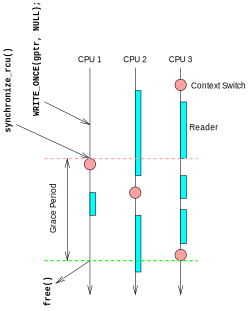
\includegraphics{defer/QSBRGracePeriod}}
\caption{QSBR\@:
		 Waiting for Pre-Existing Readers}
\label{fig:defer:QSBR: Waiting for Pre-Existing Readers}
\end{figure}

This approach is termed \IXacrfst{qsbr}~\cite{ThomasEHart2006a}.
A QSBR schematic is shown in
\cref{fig:defer:QSBR: Waiting for Pre-Existing Readers},
with time advancing from the top of the figure to the bottom.
The cyan-colored boxes depict RCU read-side critical sections,
each of which begins with \co{rcu_read_lock()} and ends with
\co{rcu_read_unlock()}.
CPU~1 does the \co{WRITE_ONCE()} that removes the current data
item (presumably having previously read the pointer value and
availed itself of appropriate synchronization), then waits
for readers.
This wait operation results in an immediate context switch, which is a
quiescent state (denoted by the pink circle), which in turn means that
all prior reads on CPU~1 have completed.
Next, CPU~2 does a context switch, so that all readers on CPUs~1 and~2
are now known to have completed.
Finally, CPU~3 does a context switch.
At this point, all readers throughout the entire system are known to have
completed, so the grace period ends, permitting \co{synchronize_rcu()} to
return to its caller, in turn permitting CPU~1 to free the old data item.

\QuickQuiz{
	In \cref{fig:defer:QSBR: Waiting for Pre-Existing Readers},
	the last of CPU~3's readers that could possibly have
	access to the old data item ended before the grace period
	even started!
	So why would anyone bother waiting until CPU~3's later context
	switch???
}\QuickQuizAnswer{
	Because that waiting is exactly what enables readers to use
	the same sequence of instructions that is appropriate for
	single-theaded situations.
	In other words, this additional ``redundant'' waiting enables
	excellent read-side performance, scalability, and real-time
	response.
}\QuickQuizEnd

\subsubsection{Toy Implementation}
\label{sec:defer:Toy Implementation}

Although production-quality QSBR implementations can be quite complex,
a toy non-preemptive Linux-kernel implementation is exceedingly simple:

\begin{VerbatimN}[samepage=true]
void synchronize_rcu(void)
{
	int cpu;

	for_each_online_cpu(cpu)
		sched_setaffinity(current->pid, cpumask_of(cpu));
}
\end{VerbatimN}

The \co{for_each_online_cpu()} primitive iterates over all CPUs, and
the \co{sched_setaffinity()} function causes the current thread to
execute on the specified CPU, which forces the destination CPU to execute
a context switch.
Therefore, once the \co{for_each_online_cpu()} has completed, each CPU
has executed a context switch, which in turn guarantees that
all pre-existing reader threads have completed.

\begin{listing}
\begin{fcvlabel}[ln:defer:Insertion and Deletion With Concurrent Readers]
\begin{VerbatimL}[commandchars=\\\[\]]
struct route *gptr;

int access_route(int (*f)(struct route *rp))
{
	int ret = -1;
	struct route *rp;

	rcu_read_lock();
	rp = rcu_dereference(gptr);
	if (rp)
		ret = f(rp);		\lnlbl[access_rp]
	rcu_read_unlock();
	return ret;
}

struct route *ins_route(struct route *rp)
{
	struct route *old_rp;

	spin_lock(&route_lock);
	old_rp = gptr;
	rcu_assign_pointer(gptr, rp);
	spin_unlock(&route_lock);
	return old_rp;
}

int del_route(void)
{
	struct route *old_rp;

	spin_lock(&route_lock);
	old_rp = gptr;
	RCU_INIT_POINTER(gptr, NULL);
	spin_unlock(&route_lock);
	synchronize_rcu();
	free(old_rp);
	return !!old_rp;
}
\end{VerbatimL}
\end{fcvlabel}
\caption{Insertion and Deletion With Concurrent Readers}
\label{lst:defer:Insertion and Deletion With Concurrent Readers}
\end{listing}

Please note that this approach is \emph{not} production quality.
Correct handling of a number of corner cases and the need for a number
of powerful optimizations mean that production-quality implementations
are quite complex.
In addition, RCU implementations for preemptible environments
require that readers actually do something, which in non-real-time
Linux-kernel environments can be as simple as defining
\co{rcu_read_lock()} and \co{rcu_read_unlock()} as \co{preempt_disable()}
and \co{preempt_enable()}, respectively.\footnote{
	Some toy RCU implementations that handle preempted
	read-side critical sections are shown in
	\cref{chp:app:``Toy'' RCU Implementations}\@.}
However, this simple non-preemptible approach is conceptually complete,
and demonstrates that it really is possible to provide read-side
synchronization at zero cost, even in the face of concurrent updates.
In fact,
\cref{lst:defer:Insertion and Deletion With Concurrent Readers}
shows how reading (\co{access_route()}),
\cref{fig:defer:Insertion With Concurrent Readers}'s
insertion (\co{ins_route()}) and
\cref{fig:defer:Deletion With Concurrent Readers}'s
deletion (\co{del_route()}) can
be implemented.
(A slightly more capable routing table is shown in
\cref{sec:defer:RCU for Pre-BSD Routing}.)

\QuickQuizSeries{%
\QuickQuizB{
	What is the point of \co{rcu_read_lock()} and \co{rcu_read_unlock()} in
	\cref{lst:defer:Insertion and Deletion With Concurrent Readers}?
	Why not just let the quiescent states speak for themselves?
}\QuickQuizAnswerB{
	Recall that readers are not permitted to pass through a quiescent
	state.
	For example, within the Linux kernel, RCU readers are not permitted
	to execute a context switch.
	Use of \co{rcu_read_lock()} and \co{rcu_read_unlock()} enables
	debug checks for improperly placed quiescent states, making it
	easy to find bugs that would otherwise be difficult to find,
	intermittent, and quite destructive.
}\QuickQuizEndB
%
\QuickQuizE{
	What is the point of \co{rcu_dereference()}, \co{rcu_assign_pointer()}
	and \co{RCU_INIT_POINTER()} in
	\cref{lst:defer:Insertion and Deletion With Concurrent Readers}?
	Why not just use \co{READ_ONCE()}, \co{smp_store_release()}, and
	\co{WRITE_ONCE()}, respectively?
}\QuickQuizAnswerE{
	The RCU-specific APIs do have similar semantics to the suggested
	replacements, but also enable static-analysis debugging checks
	that complain if an RCU-specific API is invoked on a non-RCU
	pointer and vice versa.
}\QuickQuizEndE
}

Referring back to
\cref{lst:defer:Insertion and Deletion With Concurrent Readers},
note that \co{route_lock} is used to synchronize between concurrent updaters
invoking \co{ins_route()} and \co{del_route()}.
However, this lock is not acquired by readers invoking \co{access_route()}:
Readers are instead protected by the QSBR techniques described in this section.

Note that \co{ins_route()} simply returns the old value of \co{gptr}, which
\cref{fig:defer:Insertion With Concurrent Readers} assumed would
always be \co{NULL}.
This means that it is the caller's responsibility to figure out what to
do with a non-\co{NULL} value, a task complicated by the fact that
readers might still be referencing it for an indeterminate period of time.
Callers might use one of the following approaches:

\begin{enumerate}
\item	Use \co{synchronize_rcu()} to safely free the pointed-to structure.
	Although this approach is correct from an RCU perspective, it
	arguably has software-engineering leaky-API problems.
\item	Trip an assertion if the returned pointer is non-\co{NULL}.
\item	Pass the returned pointer to a later invocation of
	\co{ins_route()} to restore the earlier value.
\end{enumerate}

In contrast, \co{del_route()} uses \co{synchronize_rcu()} and
\co{free()} to safely free the newly deleted data item.

\QuickQuiz{
	But what if the old structure needs to be freed, but the caller
	of \co{ins_route()} cannot block, perhaps due to performance
	considerations or perhaps because the caller is executing within
	an RCU read-side critical section?
}\QuickQuizAnswer{
	A \co{call_rcu()} function, which is described in
	\cref{sec:defer:Wait For Pre-Existing RCU Readers},
	permits asynchronous grace-period waits.
}\QuickQuizEnd

This example shows one general approach to reading and updating
RCU-protected data structures, however, there is quite a variety
of use cases, several of which are covered in
\cref{sec:defer:RCU Usage}.

In summary, it is in fact possible to create concurrent linked data
structures that can be traversed by readers executing the same sequence
of machine instructions that would be executed by single-threaded readers.
The next section summarizes RCU's high-level properties.

\subsubsection{RCU Properties}
\label{sec:defer:RCU Properties}

A key RCU property is that reads need not wait for updates.
This property enables RCU implementations to provide low-cost or even
no-cost readers, resulting in low overhead and excellent scalability.
This property also allows RCU readers and updaters to make useful
concurrent forward progress.
In contrast, conventional synchronization primitives must enforce strict
mutual exclusion using expensive instructions, thus increasing overhead
and degrading scalability, but also typically prohibiting readers and
updaters from making useful concurrent forward progress.

\QuickQuiz{
	Doesn't \cref{sec:defer:Sequence Locks}'s seqlock
	also permit readers and updaters to make useful concurrent
	forward progress?
}\QuickQuizAnswer{
	Yes and no.
	Although seqlock readers can run concurrently with
	seqlock writers, whenever this happens, the \co{read_seqretry()}
	primitive will force the reader to retry.
	This means that any work done by a seqlock reader running concurrently
	with a seqlock updater will be discarded and the redone upon retry.
	So seqlock readers can \emph{run} concurrently with updaters,
	but they cannot actually get any work done in this case.

	In contrast, RCU readers can perform useful work even in presence
	of concurrent RCU updaters.

	However, both reference counters
	(\cref{sec:defer:Reference Counting})
	and hazard pointers
	(\cref{sec:defer:Hazard Pointers})
	really do permit useful concurrent forward progress for both
	updaters and readers, just at somewhat greater cost.
	Please see
	\cref{sec:defer:Which to Choose?}
	for a comparison of these different solutions to the
	deferred-reclamation problem.
}\QuickQuizEnd

As noted earlier, RCU delimits readers with \co{rcu_read_lock()} and
\co{rcu_read_unlock()}, and ensures that each reader has a coherent view
of each object (see \cref{fig:defer:Deletion With Concurrent Readers}) by
maintaining multiple versions of objects and using update-side primitives
such as \co{synchronize_rcu()} to ensure that objects are not
freed until after the completion of all readers that might be using them.
RCU uses \co{rcu_assign_pointer()} and \co{rcu_dereference()} to provide
efficient and scalable mechanisms for publishing and reading new versions
of an object, respectively.
These mechanisms distribute the work among read and
update paths in such a way as to make read paths extremely fast, using
replication and weakening optimizations in a manner similar to
\IXpl{hazard pointer}, but without the need for read-side retries.
In some cases, including \co{CONFIG_PREEMPT=n} Linux kernels,
RCU's read-side primitives have zero overhead.

But are these properties actually useful in practice?
This question is taken up by the next section.

\subsubsection{Practical Applicability}
\label{sec:defer:Practical Applicability}

\begin{figure}
\centering
\resizebox{3in}{!}{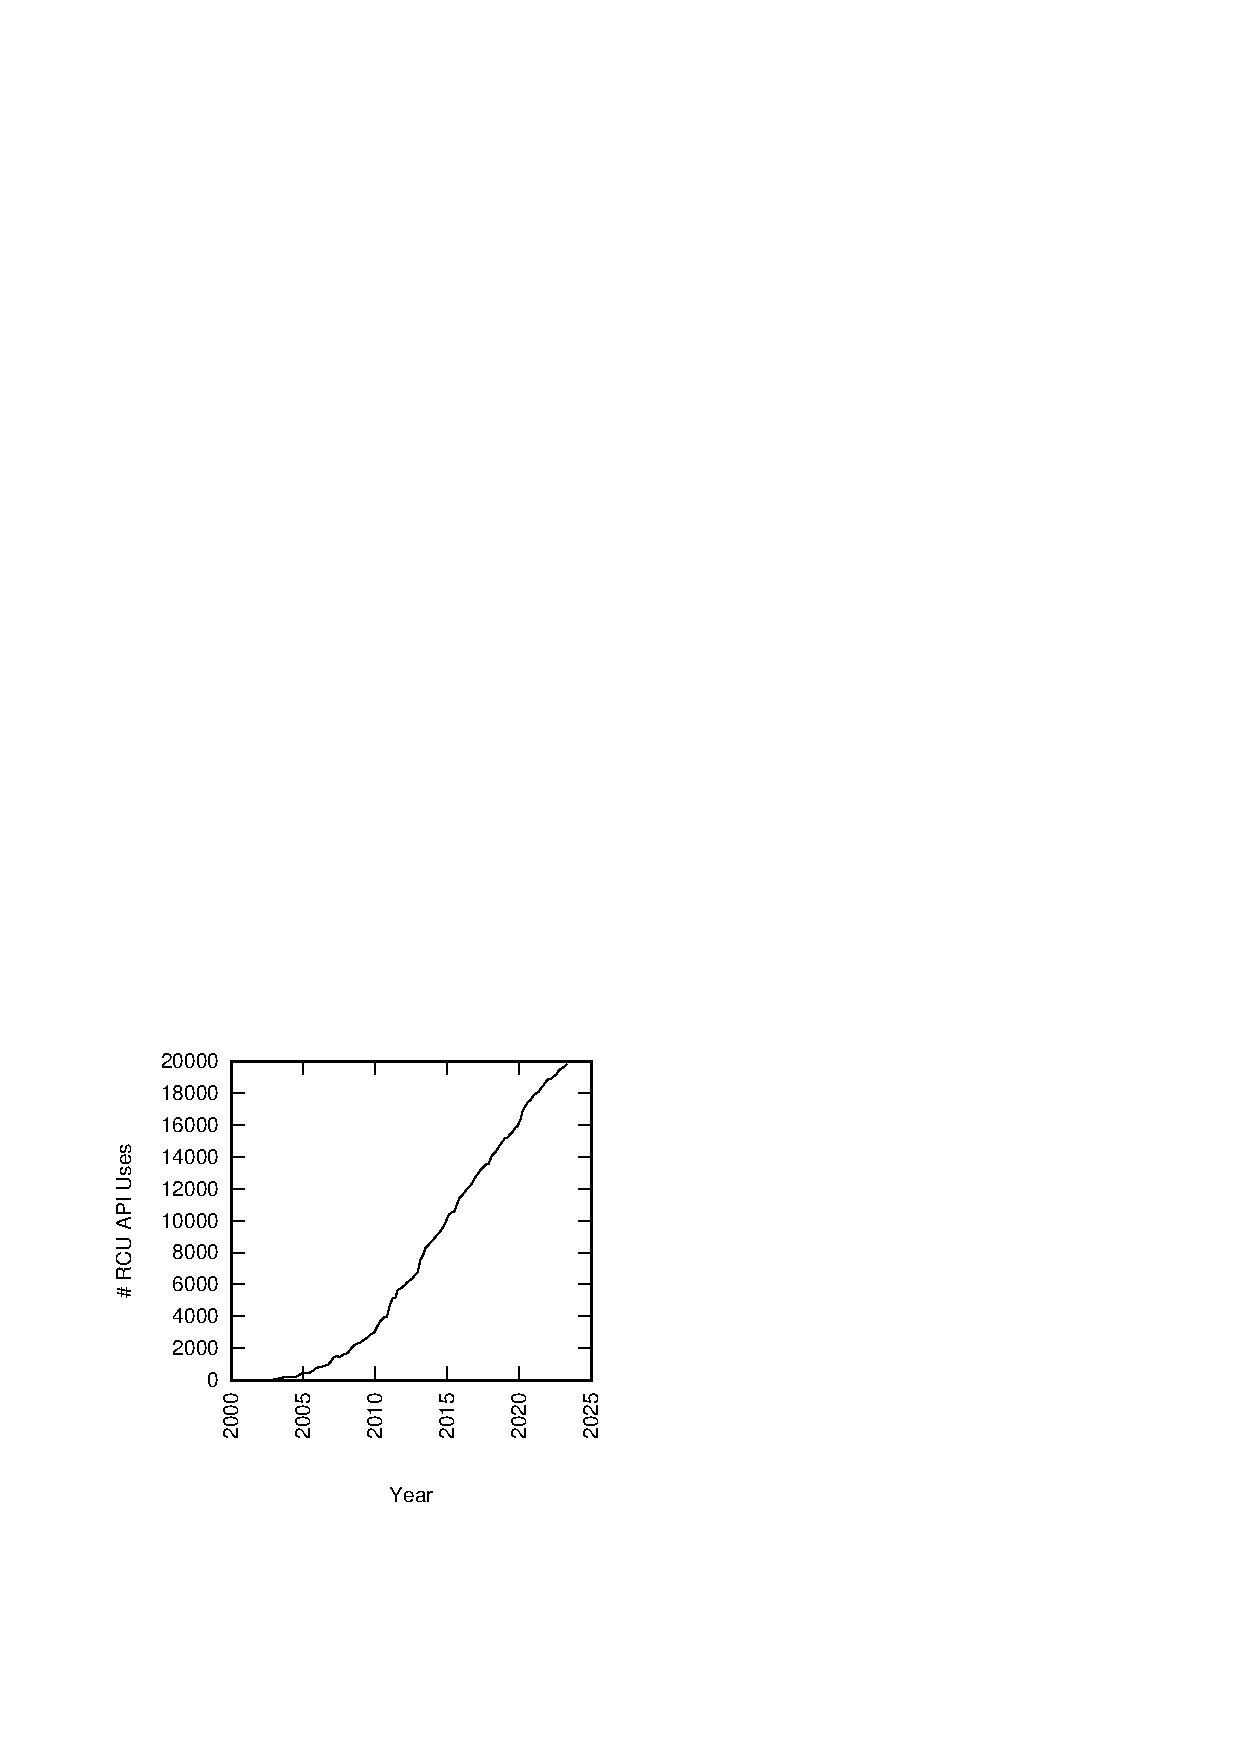
\includegraphics{defer/linux-RCU}}
\caption{RCU Usage in the Linux Kernel}
\label{fig:defer:RCU Usage in the Linux Kernel}
\end{figure}

RCU has been used in the Linux kernel since
October 2002~\cite{Torvalds2.5.43}.
Use of the RCU API has increased substantially since that time,
as can be seen in
\cref{fig:defer:RCU Usage in the Linux Kernel}.
In fact, code very similar to that in
\cref{lst:defer:Insertion and Deletion With Concurrent Readers}
is used in the Linux kernel.
RCU has enjoyed heavy use both prior to and since its acceptance
in the Linux kernel, as discussed in
\cref{sec:defer:RCU Related Work}.

It is therefore safe to say that RCU enjoys wide practical applicability.

The minimal example discussed in this section is a good introduction to RCU\@.
However, effective use of RCU often requires that you think differently
about your problem.
It is therefore useful to examine RCU's fundamentals, a task taken up
by the following section.
